\documentclass[border=12pt]{standalone}
\def\pgfsysdriver{pgfsys-dvisvgm.def}
\usepackage[dvisvgm]{xcolor}
\usepackage{xeCJK}
\setCJKmainfont{HaranoAjiGothic-Regular.otf}[BoldFont=HaranoAjiGothic-Bold.otf]
\setCJKsansfont{HaranoAjiGothic-Regular.otf}[BoldFont=HaranoAjiGothic-Bold.otf]
\usepackage{amsmath,amssymb,tikz,lmodern}
\usetikzlibrary{arrows.meta,positioning,calc,fit,backgrounds}
\renewcommand{\familydefault}{\sfdefault}
\definecolor{ink}{HTML}{25322F}
\definecolor{green}{HTML}{246657}
\definecolor{tint}{HTML}{EEF4F0}
\definecolor{soft}{HTML}{C6D2CC}
\definecolor{muted}{HTML}{52615B}
\newif\ifJapanese
\newcommand{\Tx}[2]{\ifJapanese #1\else #2\fi}
\newcommand{\Eff}{\overline{\operatorname{Eff}}}
\newcommand{\heading}[3]{{\color{green}\bfseries #1\quad\Tx{#2}{#3}}\\[5pt]}
% A white rectangle makes the complete citation label clickable, including spaces.
\newcommand{\refurl}[2]{\special{dvisvgm:raw <a xlink:href="#1" target="_blank" rel="noopener noreferrer">}{\setlength{\fboxsep}{0pt}\colorbox{white}{\color{green}\underline{\strut #2}}}\special{dvisvgm:raw </a>}}
\tikzset{
 card/.style={draw=soft,fill=white,rounded corners=2pt,align=left,text=ink,font=\fontsize{10.5}{14}\selectfont,inner xsep=12pt,inner ysep=10pt,text width=14.4cm},
 half/.style={card,text width=6.45cm,minimum height=2.05cm},
 result/.style={card,draw=green,fill=tint,line width=.9pt},
 reason/.style={align=left,text=muted,font=\fontsize{9}{12}\selectfont,inner sep=0pt,text width=12.7cm},
 branchreason/.style={reason,text width=5.95cm},
 edge/.style={-{Stealth[length=2.4mm]},draw=green,line width=1pt},
 wire/.style={draw=green,line width=1pt},
}
% Keep the arrow in a dedicated left gutter; explanations never cover it.
\newcommand{\flow}[3]{
 \coordinate (#2-from) at ($(#1.south)+(-6.9,0)$);
 \coordinate (#2-to) at ($(#2.north)+(-6.9,0)$);
 \draw[edge] (#2-from)--(#2-to);
 \node[reason,anchor=west] (#2-reason) at ($(#2-from)!.5!(#2-to)+(.55,0)$) {#3};
}

\newcommand{\Cite}[2]{\refurl{#1}{#2}}

\Japanesefalse
\begin{document}
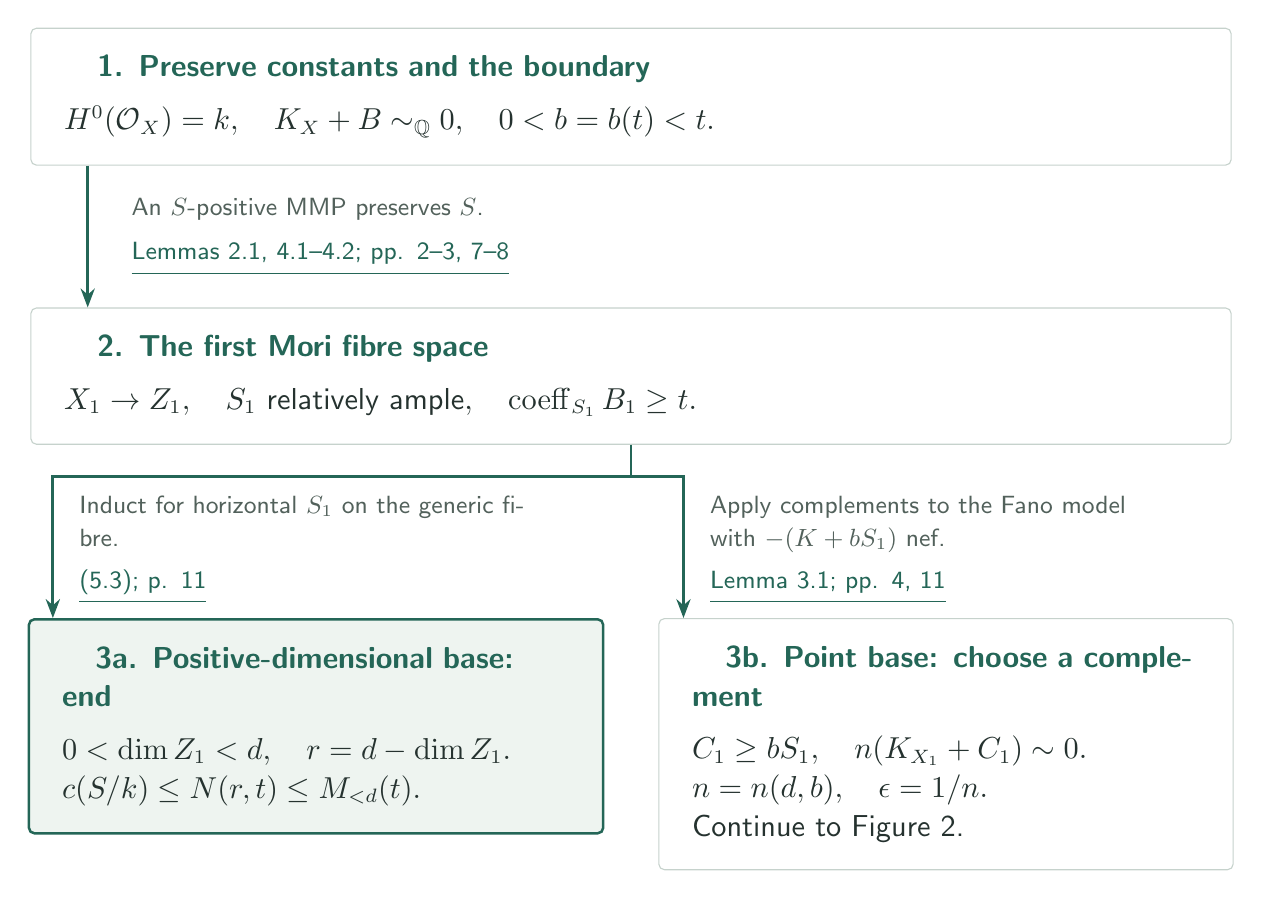
\begin{tikzpicture}
\node[card] (start) {\heading{}{1. 定数体を保って境界を残す}{1. Preserve constants and the boundary}$H^0(\mathcal O_X)=k,\quad K_X+B\sim_{\mathbb Q}0,\quad 0<b=b(t)<t.$};

\node[card,below=1.8cm of start] (mori) {\heading{}{2. 第1のMoriファイバー空間}{2. The first Mori fibre space}$X_1\to Z_1,\quad S_1\text{ relatively ample},\quad \operatorname{coeff}_{S_1}B_1\ge t.$};

\flow{start}{mori}{\Tx{$S$ に正なMMPで $S$ を保存。}{An $S$-positive MMP preserves $S$.}\\[4pt]\Cite{https://github.com/openai/math/blob/adc7f1241b42e322a6451854ab7e4b4c146bf78a/preprints/Arithmetic-Stein-degree-bounds-for-log-Calabi-Yau-pairs-September-25-2026/paper.pdf}{Lemmas 2.1, 4.1--4.2; pp. 2--3, 7--8}}
\node[result,text width=6.45cm,below=2.2cm of mori.south,xshift=-4cm] (done) {\heading{}{3a. 正次元の底：終了}{3a. Positive-dimensional base: end}$0<\dim Z_1<d,\quad r=d-\dim Z_1.$\\ $c(S/k)\le N(r,t)\le M_{<d}(t).$};

\node[half,below=2.2cm of mori.south,xshift=4cm] (next) {\heading{}{3b. 点の底：補完を選ぶ}{3b. Point base: choose a complement}$C_1\ge bS_1,\quad n(K_{X_1}+C_1)\sim0.$\\ $n=n(d,b),\quad\epsilon=1/n.$\\ \Tx{第2図へ進む。}{Continue to Figure 2.}};

\coordinate (done-a) at ($(done.north west)+(.32,0)$);
\draw[edge] (mori.south) -- ++(0,-.4) -| (done-a);
\node[branchreason,anchor=south west] at ($(done.north west)+(.65,.18)$) {\Tx{水平な $S_1$ を一般ファイバーで帰納。}{Induct for horizontal $S_1$ on the generic fibre.}\\[3pt]\Cite{https://github.com/openai/math/blob/adc7f1241b42e322a6451854ab7e4b4c146bf78a/preprints/Arithmetic-Stein-degree-bounds-for-log-Calabi-Yau-pairs-September-25-2026/paper.pdf}{(5.3); p. 11}};

\coordinate (next-a) at ($(next.north west)+(.32,0)$);
\draw[edge] (mori.south) -- ++(0,-.4) -| (next-a);
\node[branchreason,anchor=south west] at ($(next.north west)+(.65,.18)$) {\Tx{Fanoかつ $-(K+bS_1)$ nefに補完を適用。}{Apply complements to the Fano model with $-(K+bS_1)$ nef.}\\[3pt]\Cite{https://github.com/openai/math/blob/adc7f1241b42e322a6451854ab7e4b4c146bf78a/preprints/Arithmetic-Stein-degree-bounds-for-log-Calabi-Yau-pairs-September-25-2026/paper.pdf}{Lemma 3.1; pp. 4, 11}};

\end{tikzpicture}
\end{document}
